\documentclass[tikz, border=3mm]{standalone}
\usetikzlibrary{chains,decorations.pathreplacing}

\begin{document}
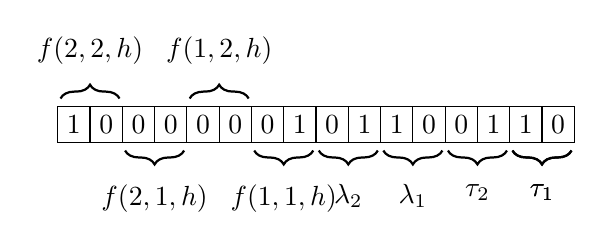
\begin{tikzpicture}[
        node distance=0pt,
        start chain = A going right,
        X/.style = {rectangle, draw,% styles of nodes in string (chain)
                minimum width=2ex, minimum height=3ex,
                outer sep=0pt, on chain},
        B/.style = {decorate,
                decoration={brace, amplitude=5pt,
                        pre=moveto,pre length=1pt,post=moveto,post length=1pt,
                        raise=1mm,
                        #1}, % for mirroring of brace, if necessary
                thick},
        B/.default=mirror, % by default braces are mirrored
    ]
    \foreach \i in {1,0,0,0,0,0,0,1,0,1,1,0,0,1,1,0} % <-- content of nodes
    \node[X] {\i};
    \draw[B] ( A-15.south west) -- node[below=4mm] {$\tau_{1}$} ( A-16.south east);
    \draw[B] ( A-15.south west) -- node[below=4mm] {$\tau_{1}$} ( A-16.south east);
    \draw[B] ( A-13.south west) -- node[below=4mm] {$\tau_{2}$} ( A-14.south east);
    \draw[B] ( A-11.south west) -- node[below=4mm] {$\lambda_{1}$} ( A-12.south east);
    \draw[B] ( A-9.south west) -- node[below=4mm] {$\lambda_{2}$} ( A-10.south east);
    \draw[B] ( A-7.south west) -- node[below=4mm] {$f(1,1,h)$} ( A-8.south east);
    \draw[B=] ( A-5.north west) -- node[above=4mm] {$f(1,2,h)$} ( A-6.north east);
    \draw[B] ( A-3.south west) -- node[below=4mm] {$f(2,1,h)$} ( A-4.south east);
    \draw[B=] ( A-1.north west) -- node[above=4mm] {$f(2,2,h)$} ( A-2.north east);
\end{tikzpicture}
\end{document}
